\documentclass[letterpaper,12pt]{article}
\usepackage{amsmath}  % improve math presentation
\usepackage{graphicx} % takes care of graphic including machinery
\usepackage{mathrsfs}


\usepackage[final]{hyperref} % adds hyper links inside the generated pdf file
\hypersetup{
	colorlinks=true,       % false: boxed links; true: colored links
	linkcolor=blue,        % color of internal links
	citecolor=blue,        % color of links to bibliography
	filecolor=magenta,     % color of file links
	urlcolor=blue         
}

\title{Sixth Assignment for Computational Physics}
\date{\today}
\author{Xinyu Liu}


\begin{document}
\maketitle
\tableofcontents

\newpage

\section{My Github Page URL}
\url{https://github.com/rising1227/phys-ga2000}

\section{Solving the Lagrange Point}

The Associated Code for this assignment is ps7-1.py.

\subsection{Theoretical derivation for the Lagrangian Point}

Here's the physical setup for the system. Since the earth has much larger mass than moon, we assume that the earth is almost not moving and the moon and satelite is orbiting around the earth.

\begin{table}[!h]
    \centering
    \caption{Physical Setup for the system}
    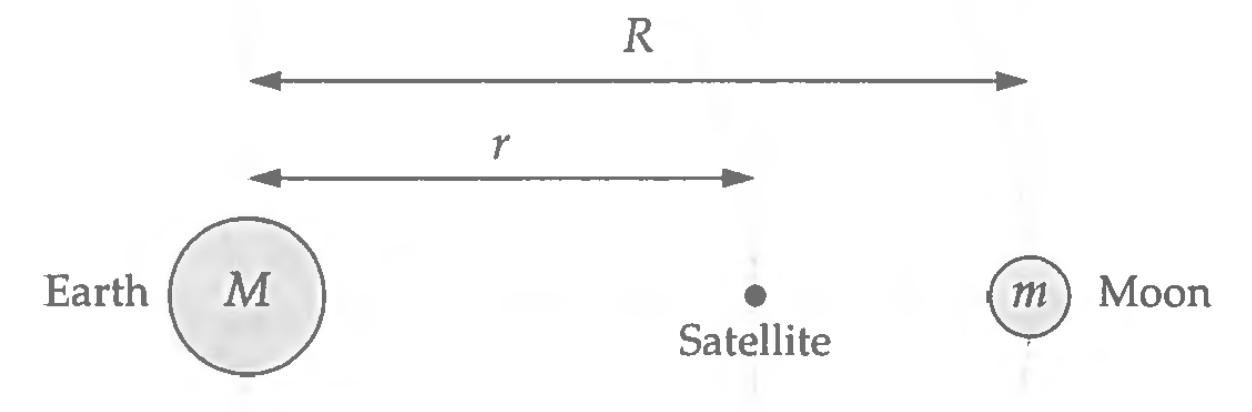
\includegraphics[width=11cm]{ps7.11.png}
\end{table}%

For the equation of motion of the satelite(with mass $m_1$), we have:

\begin{equation}
    m_1 \omega^2 r = \frac{GMm_1}{r^2} - \frac{Gmm_1}{(R-r)^2}
\end{equation}

From the two-body motion of moon orbiting around the earth, we have:

\begin{equation}
    \omega^2 = \frac{G(M+m)}{R^3}
\end{equation}

So that, the lagrange point r satisfies:

\begin{equation}
    m_1\frac{G(M+m)}{R^3}r = \frac{GMm_1}{r^2} - \frac{Gmm_1}{(R-r)^2}
\end{equation}

Finally:

\begin{equation}
    \frac{M+m}{R^3}r = \frac{M}{r^2} - \frac{m}{(R-r)^2}
\end{equation}

By defining dimensionless parameter $m' = m/M$ and $r' = r/R$, the function for $r'$ goes to:

\begin{equation}
    (1+m')r' = \frac{1}{r'^2} - \frac{m'}{(1-r')^2}
\end{equation}

By rewriting the function:

\begin{equation}
    f(m',r') = (1+m')r'^3 (1-r')^2 - (1-r')^2 + m' r'^2 = 0
\end{equation}

For a physical problem, we generally have a fixed m' and would like to solve the lagrange point position r', which is a fifth order equation and need to be solved numerically.

\subsection{Using Newton Method to Solve the Equation Numerically}

In the code we numerically carried out the newton method. From the description of Newman 6.16, we are here more interested in the lagrangian point between two planets. We defined the previous function $f(m',r')$ and its derivative against r' analytically. Then we start from trying $x = 1$ and converge to the solution by iterating $x_{i+1} = x_i - \frac{f(x_i)}{f'(x_i)}$. The iteration stops when the accuracy $f(x') < 10^{-10}$ is reached. We found out that:

\begin{itemize}
    \item For the Moon and the Earth case: $r' = 0.8479712150055999$, $r = R_{em}r' = 3.25963 * 10^8 m$
    \item For the Earth and the Sun case: $r' = 0.9900302345297135$, $r = R_{es}r' = 1.48106 * 10^{11} m$
    \item For a Jupiter-mass planet orbiting the Sun at the distance of the Earth case: $r' = 0.9332336787481736$, $r = R_{es}r' = 1.39610 * 10^{11} m$
\end{itemize}



\section{Implementing Brent 1D minimization method}

The Associated Code for this assignment is ps7-2.py.

We carried out the Brent's minimization method described by the book. Essentially, we broadly choose two starting point to form the bracket and use the golden selection search to find a midpoint. We then use parabolic estimation to search for a minimization point. If this parabolic estimation give a reasonable searching point, we compare its value with the midpoint and form a new bracket. Otherwise, we use golden search rule to find new bracket. The iteration continues until the function value cannot be minimized to a certain order($10^{-10}$).

In our program, we set the initial bracket to be from -2 to 2 and we successfully searched out the minimal value point $x_3 = 0.299990501074631$.

However, we also tried the scipy.optimize.brent method. We found out that whether it can search out the minimal value point $x_3 = 0.300000000023735$ which is similar to our result.

\end{document}